

\documentclass[a4paper]{scrartcl}

\usepackage[utf8]{inputenc}
\usepackage[english]{babel}
\usepackage{lmodern} 
\usepackage[T1]{fontenc}
\usepackage{booktabs}
\usepackage{multirow}
\usepackage{wrapfig}


% PAKETE
\usepackage{siunitx}
\usepackage{graphicx}
\usepackage{placeins}
\usepackage{longtable}
\usepackage{enumitem}
\usepackage{bbm}
%\usepackage{sidecap}


\usepackage{amssymb} % math symbols
\usepackage{amsmath} % ams
\usepackage{amsfonts} % mathmatical fonts

% caption indenting
 \usepackage[format=plain,indention=0em,labelfont=bf,margin=1em]{caption} 
 \usepackage{subfig} %subfigures ^^
\usepackage[protrusion=true,expansion=true]{microtype} % denser font, "-" behind line
\usepackage{esint} % nicer double and triple integrals
\usepackage{fancyhdr} % fancy headers
\usepackage[colorlinks=true,linkcolor=black,citecolor=black,filecolor=black,urlcolor=black]{hyperref}



% EINSTELLUNGEN
\sisetup{seperr,repeatunits=false}
\numberwithin{equation}{section}
\numberwithin{figure}{section}
\numberwithin{table}{section}

% EIGENE FUNKTIONEN
\newcommand{\re}{\operatorname{Re}}
\newcommand{\im}{\operatorname{Im}}
\newcommand{\gquote}[1]{\glqq #1 \grqq}

\newcommand{\eq}[2]{\begin{equation}#1\label{#2}\end{equation}}
\newcommand{\eqand}[0]{\hspace{.25cm} \bigwedge \hspace{.25cm}}
\newcommand{\grafik}[2]{\begin{figure}[h]\centering \includegraphics[width=10cm]{#1.eps}  \caption{#2} \label{#1} \end{figure} }
\newcommand{\grafikq}[3]{\begin{figure}[h]\centering \includegraphics[width=10cm]{#1.eps}  \caption[#2]{#3} \label{#1} \end{figure} }
\newcommand{\tbl}[3]{\begin{table}[h]\caption{#1}\label{#2}\begin{center}#3\end{center}\end{table}}
\newcommand{\Abbildung}[1]{\textsl{Abbildung \ref{#1}}}
\newcommand{\AbbildungI}[1]{\textsl{(Abbildung \ref{#1})}}
\newcommand{\Tabelle}[1]{\textsl{Tabelle \ref{#1}}}
\newcommand{\TabelleI}[1]{\textsl{(Tabelle \ref{#1})}}
\newcommand{\Formel}[1]{(\ref{#1})}
\renewcommand{\d}{\mathrm{d}}
\newcommand{\ve}[1]{\mathbf{ #1} }



\begin{document}
\section*{Superconductivity}
\small
\subsection*{Historical Overview}
Superconductivity was found experimentally in 1911 by H. Kammerlingh Onnes. The liquidation of helium made experiments below $T=4$ K possible. Onnes investigated the electrical resistivity of metals, which was believed to decrease with temperature smoothly as the oscillation of the lattice atoms decline. It was predicted that it reaches a finite value at zero temperature due to impurities of the metal, instead for various materials the rapid decay of resistivity at a certain temperature $T_C$ was detected \ref{fig:onnes}. 

\begin{wrapfigure}{r}{0.3\linewidth}
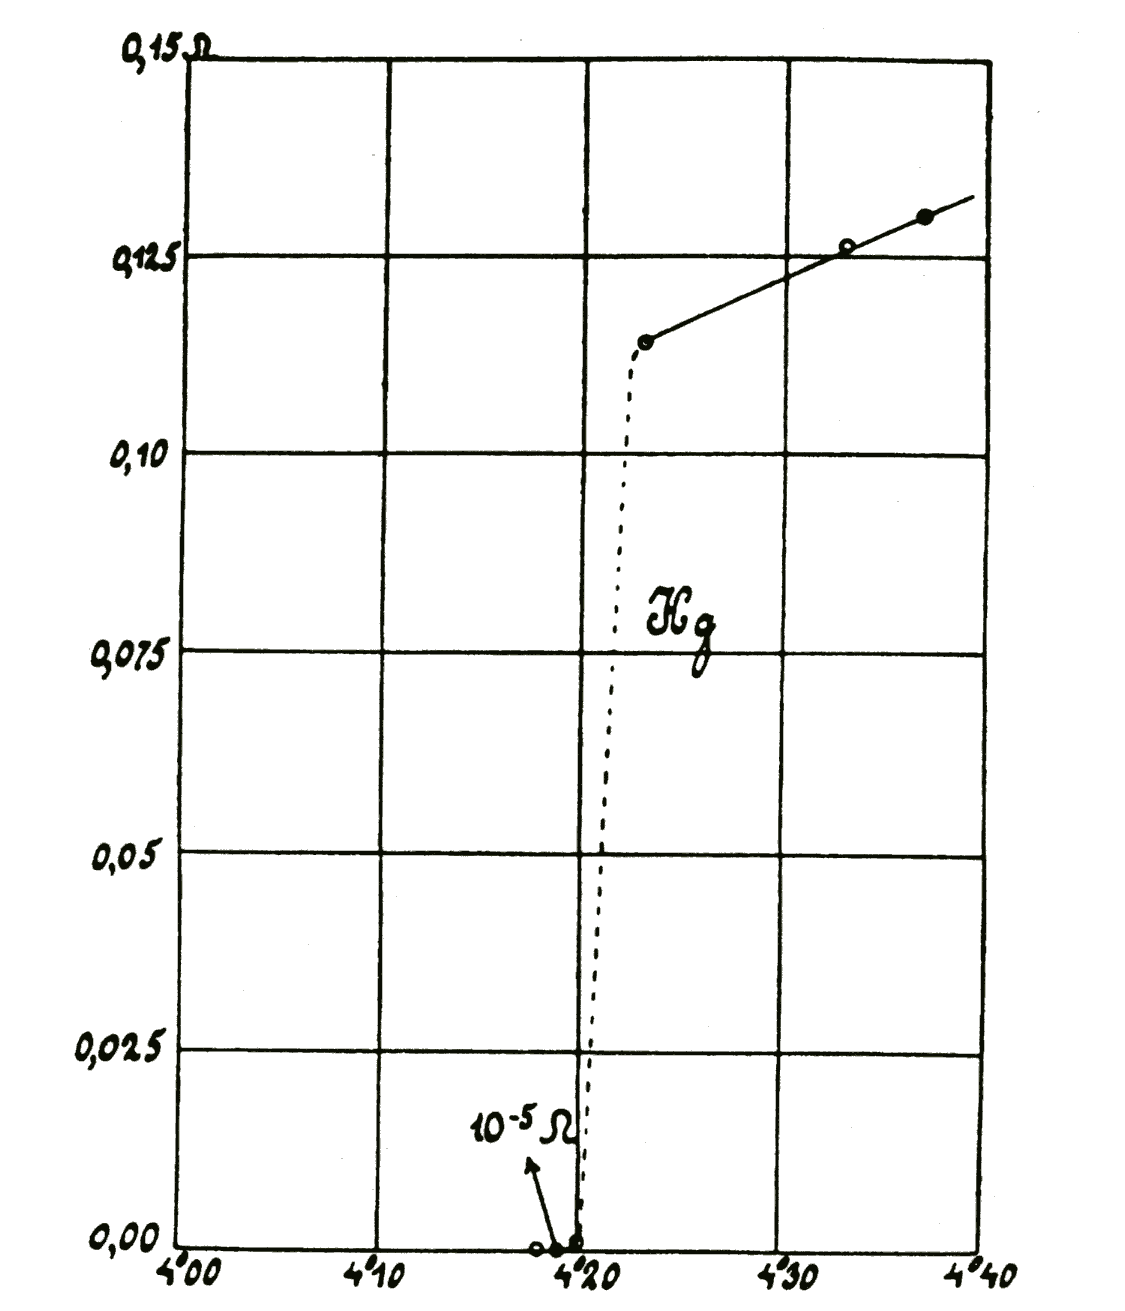
\includegraphics[width=0.3\textwidth]{img/heikemess.png}
\caption{\small Original Data for Mercury (Onnes, 1911) \cite{onnes}}
\label{fig:onnes}
\end{wrapfigure}

The first phenomenological theory of superconductivity was developed by the brothers F. and H. London in 1935 after the discovery of the Meißner-Ochsenfeld Effect in 1933 and during the 1950s the more elaborate Ginsburg-Landau-Theory was developed. In 1957 Bardeen, Schriefer and Cooper published their famous paper on a microscopic description of superconductivity, the BCS Theory.

\subsection*{Properties of Superconductors}
The superconducting state is a new phase of matter and therefore has many new characteristics. The most important feature is the loss of electrical resistivity. Furthermore, there are three distinct critical values, which lead to the destruction of perfect conduction. These are critical temperatures, critical magnetic fields and critical electric currents. The destruction of superconductivity by all three cab be explained by the BCS theory and is linked to the binding energy of the Cooper pairs. Further remarkable properties are the quantized magnetic fluxes in certain sample geometries (e.g. rings). The energy gap of superconductors is also a very prominent feature and leads to phenomena such as the Josephson currents, which have great application in very sensitive electronical devices (SQUIDs). 

\subsection*{Meißner-Ochsenfeld Effect}
For a hypothetic material, which becomes perfectly conducting below certain magnetic fields and temperatures, it would be possible to create different phase states depending on the path, that is chosen to undergo a phase transition in the T-B-diagram (see fig \ref{fig:tb}). Activating a magnetic field during the non perfectly conducting phase and cooling down afterwards, should lead to magnetic flux inside the material. However, this is not the case for superconductors. Instead, it is an outstanding property of the superconducting phase, that all magnetic flux is expelled from the interior of the sample. This effect is called the Meißner-Ochsenfeld Effect.

\begin{wrapfigure}{r}{0.45\linewidth}
\subfloat[][]
	{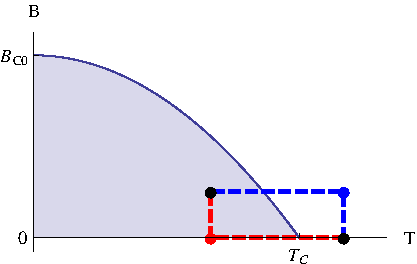
\includegraphics[width=0.3\textwidth]{img/tb6.pdf}}
\subfloat[][]
	{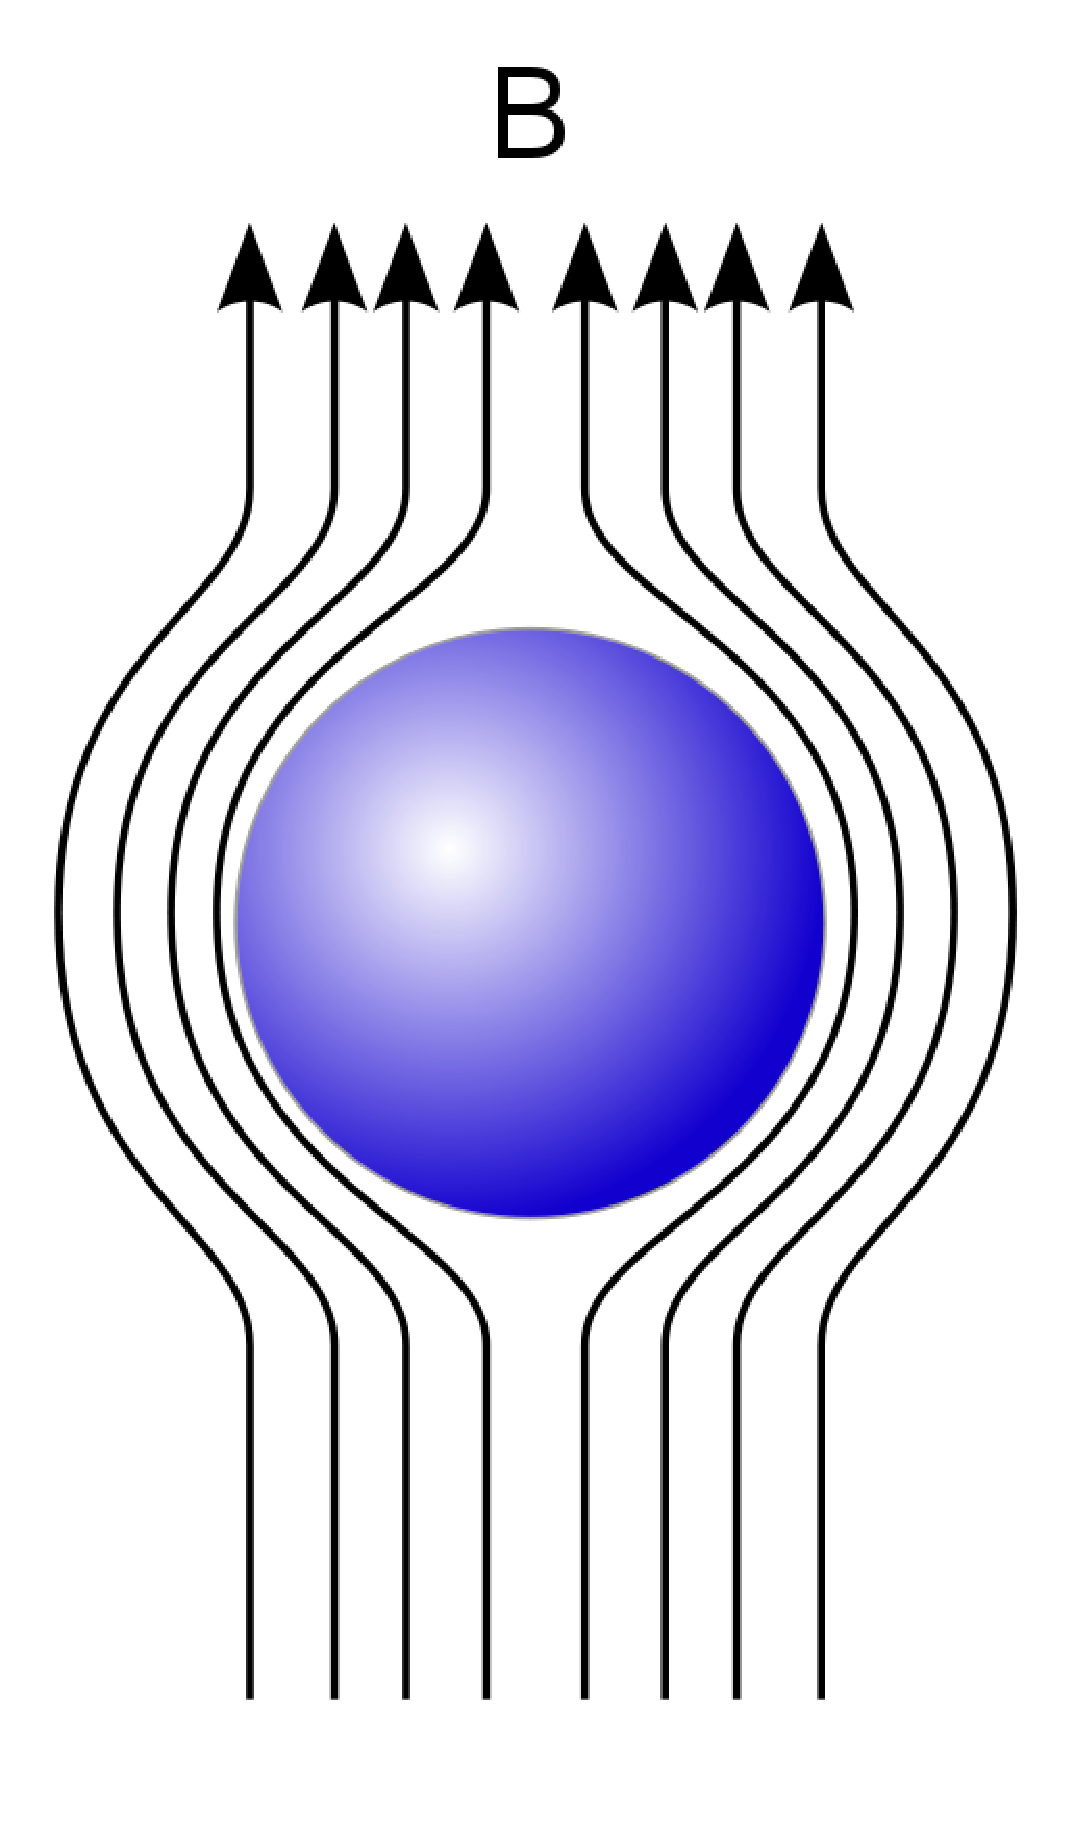
\includegraphics[width=0.15\textwidth]{img/nichdurch.pdf}}
\caption{\small \textbf{a)} Phase Transitions in the T-B-diagram. \textbf{b)} Meißner-Ochsenfeld Effect}
\label{fig:tb}
\end{wrapfigure}

\subsection*{Experiment} 
The critical temperature and the critical magnetic field of tin and indium shall be measured using the property of vanishing magnetic permeability in the superconducting phase. The permeability is measured using an electronic circuit similar to a transformer. A second induction system operated at the same voltage is used as a reference system. The whole set-up is placed within an cryogenic set-up, build by two vacuum separated and silvered cryostats. The outer dewar is filled with liquid nitrogen and the inner one with liquid helium. The pressure of the helium is tunable with a pump and is used to regulate the temperature measured through the vapor-pressure. A long coil is used to generate an external magnetic field.

\end{document}